\documentclass[../report/report.tex]{subfiles}
\begin{document}
\def\layersep{2.5cm}

\begin{figure}[!h]
\begin{center}
\begin{tikzpicture}[shorten >=1pt,->,draw=black!50, node distance=\layersep]
    \tikzstyle{every pin edge}=[<-,shorten <=1pt]
    \tikzstyle{neuron}=[circle,fill=black!25,minimum size=17pt,inner sep=0pt]
    \tikzstyle{input neuron}=[neuron, fill=blue!50];
    \tikzstyle{hidden neuron}=[neuron, fill={rgb:black,1;white,2}];
    \tikzstyle{annot} = [text width=4em, text centered]


\draw[] (1.5,3) node {\Large{Restricted Boltzmann Machine}};
    % Draw the input layer nodes
    \foreach \name / \y in {1,...,4}
    % This is the same as writing \foreach \name / \y in {1/1,2/2,3/3,4/4}
        \node[input neuron, pin=left:Input \y] (I-\name) at (0,-\y) {};

    % Draw the hidden layer nodes
    \foreach \name / \y in {1,...,5}
        \path[yshift=0.5cm]
            node[hidden neuron] (H-\name) at (\layersep,-\y cm) {};


    % Connect every node in the input layer with every node in the
    % hidden layer.
    \foreach \source in {1,...,4}
        \foreach \dest in {1,...,5}
            \path (I-\source) edge (H-\dest);
            
        % Annotate the layers
    \node[annot,above of=H-1, node distance=1.2cm] (hl) {Hidden layer};
    \node[annot,left of=hl] {Input layer};
\end{tikzpicture}
  \label{fig:rbm}
  \caption[1]{Performance of the systems with three possible Filterbank parametrisations.}
  \end{center}
\end{figure}

\begin{figure}[!h]
\begin{center}
\begin{tikzpicture}[shorten >=1pt,->,draw=black!50, node distance=\layersep]
    \tikzstyle{every pin edge}=[<-,shorten <=1pt]
    \tikzstyle{neuron}=[circle,fill=black!25,minimum size=17pt,inner sep=0pt]
    \tikzstyle{input neuron}=[neuron, fill=blue!50];
    \tikzstyle{hidden neuron}=[neuron, fill={rgb:black,1;white,2}];
    \tikzstyle{annot} = [text width=4em, text centered]

    % Draw the input layer nodes
    \foreach \name / \y in {1,...,4}
    % This is the same as writing \foreach \name / \y in {1/1,2/2,3/3,4/4}
        \node[input neuron, pin=left:Input \y] (I-\name) at (0,-\y) {};

    % Draw the hidden layer nodes
    \foreach \name / \y in {1,...,5}
        \path[yshift=0.5cm]
            node[hidden neuron] (H-\name) at (\layersep,-\y cm) {};


    % Connect every node in the input layer with every node in the
    % hidden layer.
    \foreach \source in {1,...,4}
        \foreach \dest in {1,...,5}
            \path (I-\source) edge (H-\dest);
            
        % Annotate the layers
    \node[annot,above of=H-1, node distance=1.2cm] (hl) {Hidden layer};
    \node[annot,left of=hl] {Input layer};

\foreach \source in {1,...,4}
        \foreach \dest in {1,...,4}
             \ifthenelse{\equal{\source}{\dest}}
        {}
        {\path (I-\source) edge[bend right] (I-\dest)};
            
   

\foreach \source in {1,...,5}
        \foreach \dest in {1,...,5}
        \ifthenelse{\equal{\source}{\dest}}
        {}
        {\path (H-\source) edge[bend right] (H-\dest)};
\end{tikzpicture}
\end{center}
  \label{fig:bm}
\end{figure}

\begin{figure}[!h]
\begin{center}
\begin{tikzpicture}[shorten >=1pt,->,draw=black!50, node distance=\layersep]
    \tikzstyle{every pin edge}=[<-,shorten <=1pt]
    \tikzstyle{neuron}=[circle,fill=black!25,minimum size=17pt,inner sep=0pt]
    \tikzstyle{input neuron}=[neuron, fill=green!50];
    \tikzstyle{output neuron}=[neuron, fill=red!50];
    \tikzstyle{hidden neuron}=[neuron, fill=blue!50];
    \tikzstyle{annot} = [text width=4em, text centered]

    % Draw the input layer nodes
    \foreach \name / \y in {1,...,4}
    % This is the same as writing \foreach \name / \y in {1/1,2/2,3/3,4/4}
        \node[input neuron, pin=left:Input \#\y] (I-\name) at (0,-\y) {};

    % Draw the hidden layer nodes
    \foreach \name / \y in {1,...,5}
        \path[yshift=0.5cm]
            node[hidden neuron] (H-\name) at (\layersep,-\y cm) {};

    % Draw the output layer node
    \node[output neuron,pin={[pin edge={->}]right:Output}, right of=H-3] (O) {};

    % Connect every node in the input layer with every node in the
    % hidden layer.
    \foreach \source in {1,...,4}
        \foreach \dest in {1,...,5}
            \path (I-\source) edge (H-\dest);

    % Connect every node in the hidden layer with the output layer
    \foreach \source in {1,...,5}
        \path (H-\source) edge (O);

    % Annotate the layers
    \node[annot,above of=H-1, node distance=1cm] (hl) {Hidden layer};
    \node[annot,left of=hl] {Input layer};
    \node[annot,right of=hl] {Output layer};
\end{tikzpicture}
  \label{fig:neuralnet}

\end{center}
\end{figure}

\newpage
\begin{figure}[!h]
\begin{center}
\begin{tikzpicture}[shorten >=1pt,->,draw=black!50, node distance=\layersep]
    \tikzstyle{every pin edge}=[<-,shorten <=1pt]
    \tikzstyle{neuron}=[circle,fill=black!25,minimum size=17pt,inner sep=0pt]
    \tikzstyle{input neuron}=[neuron, fill=blue!50];
    \tikzstyle{output neuron}=[neuron, fill=red!50];
    \tikzstyle{hidden neuron}=[neuron, fill=blue!50];
     \tikzstyle{shidden neuron}=[neuron, fill=blue!50];
          \tikzstyle{thidden neuron}=[neuron, fill=black!50];
    \tikzstyle{annot} = [text width=4em, text centered]

    % Draw the input layer nodes
    \foreach \name / \y in {1,...,3}
    % This is the same as writing \foreach \name / \y in {1/1,2/2,3/3,4/4}       
     \node[input neuron, pin=left:Input \#\y] (I-\name) at (0,-\y) {};

    % Draw the hidden layer nodes
    \foreach \name / \y in {1,...,4}
        \path[yshift=0.5cm]
            node[hidden neuron] (H-\name) at (\layersep,-\y cm) {};

    % Draw the SECOND hidden layer nodes
    \foreach \name / \y in {1,...,4}
        \path[yshift=0.5cm]
            node[shidden neuron] (S-\name) at (2*\layersep,-\y cm) {};
            
            
    % Draw the THIRD hidden layer nodes
    \foreach \name / \y in {1,...,4}
        \path[yshift=0.5cm]
            node[thidden neuron] (T-\name) at (3*\layersep,-\y cm) {};

%    % Draw the output layer node
%    \node[output neuron,pin={[pin edge={->}]right:Output}, right of=S-3] (O) {};

    % Connect every node in the input layer with every node in the
    % hidden layer.
    \foreach \source in {1,...,3}
        \foreach \dest in {1,...,4}
            \path (I-\source) edge (H-\dest);
            
% Connect every node in the hidden layer with every node in the
    % SECOND hidden layer.
    \foreach \source in {1,...,4}
        \foreach \dest in {1,...,4}
            \path (H-\source) edge (S-\dest);

% Connect every node in the hidden layer with every node in the
    % SECOND hidden layer.
    \foreach \source in {1,...,4}
        \foreach \dest in {1,...,4}
            \path (S-\source) edge (T-\dest);
            
%    % Connect every node in the hidden layer with the output layer
%    \foreach \source in {1,...,5}
%        \path (H-\source) edge (O);

    % Annotate the layers
    \node[annot,above of=H-1, node distance=1cm] (hl) {1th Hidden layer};
    \node[annot,left of=hl] {Input layer};
        \node[annot,above of=S-1, node distance=1cm] (hl) {2nd Hidden layer};
    \node[annot,above of=T-1, node distance=1cm] (hl) {3rd Hidden layer};
\end{tikzpicture}
  \label{fig:neuralnet}
  \caption[1]{}
\end{center}
\end{figure}


\begin{figure}[!h]
\begin{center}
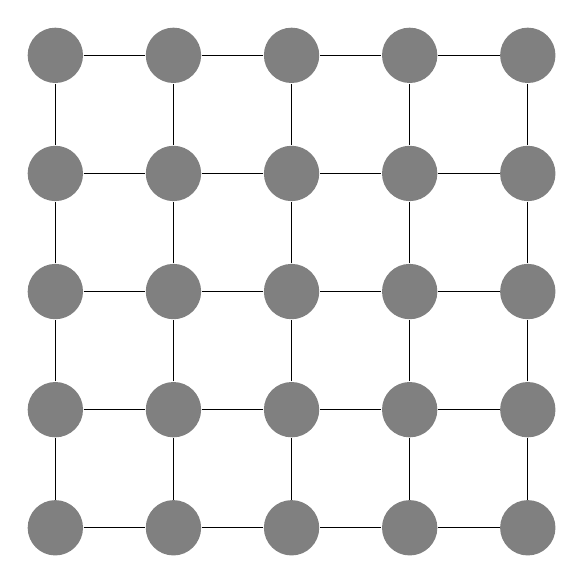
\begin{tikzpicture}[darkstyle/.style={circle,fill=black!50,minimum size=20}]
% nodes
  \foreach \x in {0,...,4}
    \foreach \y in {0,...,4} 
       {\pgfmathtruncatemacro{\label}{\x - 5 *  \y +21}
       \node [darkstyle]  (\x\y) at (1.5*\x,1.5*\y) {};} 

% connections
  \foreach \x in {0,...,4}
    \foreach \y [count=\yi] in {0,...,3}  
      \draw (\x\y)--(\x\yi) (\y\x)--(\yi\x) ;

\end{tikzpicture}
  \label{fig:neuralnet}
  \caption[1]{}
\end{center}
\end{figure}



\begin{figure}[!h]
\begin{center}
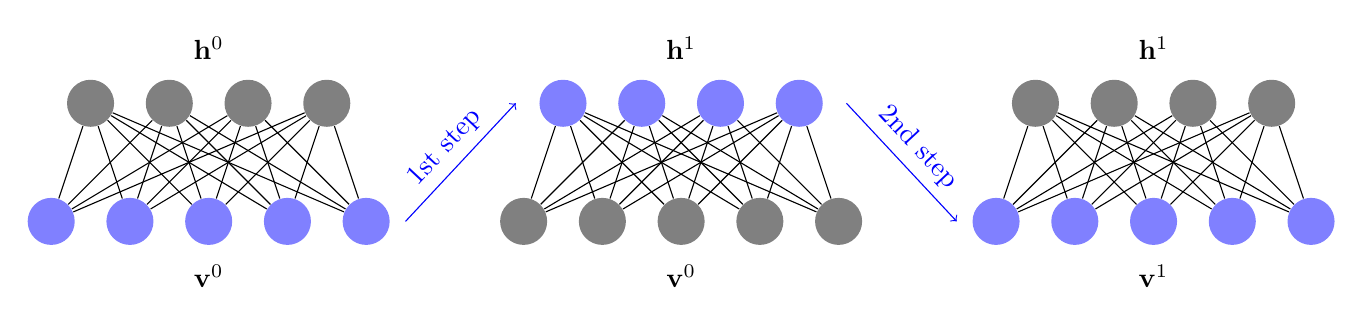
\begin{tikzpicture}[darkstyle/.style={circle,fill=black!50,minimum size=20}]
    \tikzstyle{every pin edge}=[<-,shorten <=1pt]
    \tikzstyle{neuron}=[circle,fill=black!25,minimum size=17pt,inner sep=0pt]
    \tikzstyle{input neuron}=[neuron, fill=blue!50];
    \tikzstyle{hidden neuron}=[neuron, fill=black!50];
     \tikzstyle{shidden neuron}=[neuron, fill=blue!50];
          \tikzstyle{thidden neuron}=[neuron, fill=black!50];
    \tikzstyle{annot} = [text width=4em, text centered]

    % Draw the input layer nodes
    \foreach \name / \y in {1,...,5}
    % This is the same as writing \foreach \name / \y in {1/1,2/2,3/3,4/4}       
     \node[input neuron] (I-\name) at (-\y, 0) {};

    % Draw the hidden layer nodes
\foreach \name / \y in {1,...,4}
	\node[hidden neuron] (H-\name) at (-\y -.5, 1.5) {};

    \foreach \source in {1,...,5}
        \foreach \dest in {1,...,4}
            \path (I-\source) edge (H-\dest);
            
            
    % Draw the input layer nodes
    \foreach \name / \y in {1,...,5}
    % This is the same as writing \foreach \name / \y in {1/1,2/2,3/3,4/4}       
     \node[hidden neuron] (II-\name) at (-\y +6, 0) {};

    % Draw the hidden layer nodes
\foreach \name / \y in {1,...,4}
	\node[input neuron] (HH-\name) at (-\y -.5 +6, 1.5) {};

    \foreach \source in {1,...,5}
        \foreach \dest in {1,...,4}
            \path (II-\source) edge (HH-\dest);
            
% Draw the input layer nodes
    \foreach \name / \y in {1,...,5}
    % This is the same as writing \foreach \name / \y in {1/1,2/2,3/3,4/4}       
     \node[input neuron] (III-\name) at (-\y +12, 0) {};

    % Draw the hidden layer nodes
\foreach \name / \y in {1,...,4}
	\node[hidden neuron] (HHH-\name) at (-\y -.5 +12, 1.5) {};

    \foreach \source in {1,...,5}
        \foreach \dest in {1,...,4}
            \path (III-\source) edge (HHH-\dest);
            
            \draw[->, blue] (-.5,0) -- node[above,sloped] {1st step} (.9,1.5);
                \draw[->, blue] (-.9 + 6,1.5)-- node[above,sloped] {2nd step} (.5 + 6,0);
             
            \draw    (-3,-.7) node {$\mathbf{v}^{0}$};
            \draw    (-3,2.2) node {$\mathbf{h}^{0}$};
            \draw    (-3 + 6,-.7) node {$\mathbf{v}^{0}$};
            \draw    (-3 +6,2.2) node {$\mathbf{h}^{1}$};
            \draw    (-3+ 12,-.7) node {$\mathbf{v}^{1}$};
            \draw    (-3 +12,2.2) node {$\mathbf{h}^{1}$};
\end{tikzpicture}
  \label{fig:neuralnet}
  \caption[1]{Performance of the systems with three possible Filterbank parametrisations.}
\end{center}
\end{figure}
\end{document}